\section{Image Selection}

\label{sec:selection}

\subsection{Overview}

Roughly half a million DECam exposures cover the southern sky. Most are not suitable inputs for alert-production templates: many were taken in poor atmospheric or instrumental conditions, some suffer from tracking failures or severe optical ghosts, and the depth and image quality of the archive are highly inhomogeneous. Selecting which exposures to reprocess is therefore the first step in the campaign, and it determines both the area that can be covered and the quality of the resulting templates.

This section describes how the input exposures were chosen. In brief, the parent list of exposures comes from the curated exposure list that the DELVE team uses for DELVE DR3 (\cite{DELVE})\footnote{Note: DELVE DR3 publication is in-prep, DR2 publication is provided for reference. More information about DR3 is available from \href{https://datalab.noirlab.edu/data/delve#delve-dr3}{datalab.noirlab.edu/data/delve#delve-dr3}}; a DELVE-maintained exclusion list removes known problem exposures and CCDs, and a per-template selection step picks the best-seeing exposures for each position. Table~\ref{tab:criteria} summarizes the criteria, which are described in detail below.

\subsection{Parent exposure list from DELVE DR3}

The campaign adopted the exposure list used by DELVE to generate its DR3 catalog-level coadds. This is a different product from the DELVE image coadds released previously using the DESDM pipeline.
The input list is combined with DELVE's DECam exclude list, which compiles several classes of artifact and problem exposure into a single file. Some entries are visits or CCDs that should always be excluded, such as those affected by tracking problems. Others, notably CCDs with prominent optical ghosts, may reasonably be included or excluded depending on the use. In the ELAIS-S1 pilot, for example, two visits in which more than 30 CCDs were ghosted were dropped by hand, and the chunk production used the explicit visit-detector combinations provided by the exclusion list. The input visits per band are shown in Figure~\ref{fig:delve_vis_nomask}.

\begin{figure}
    \centering
    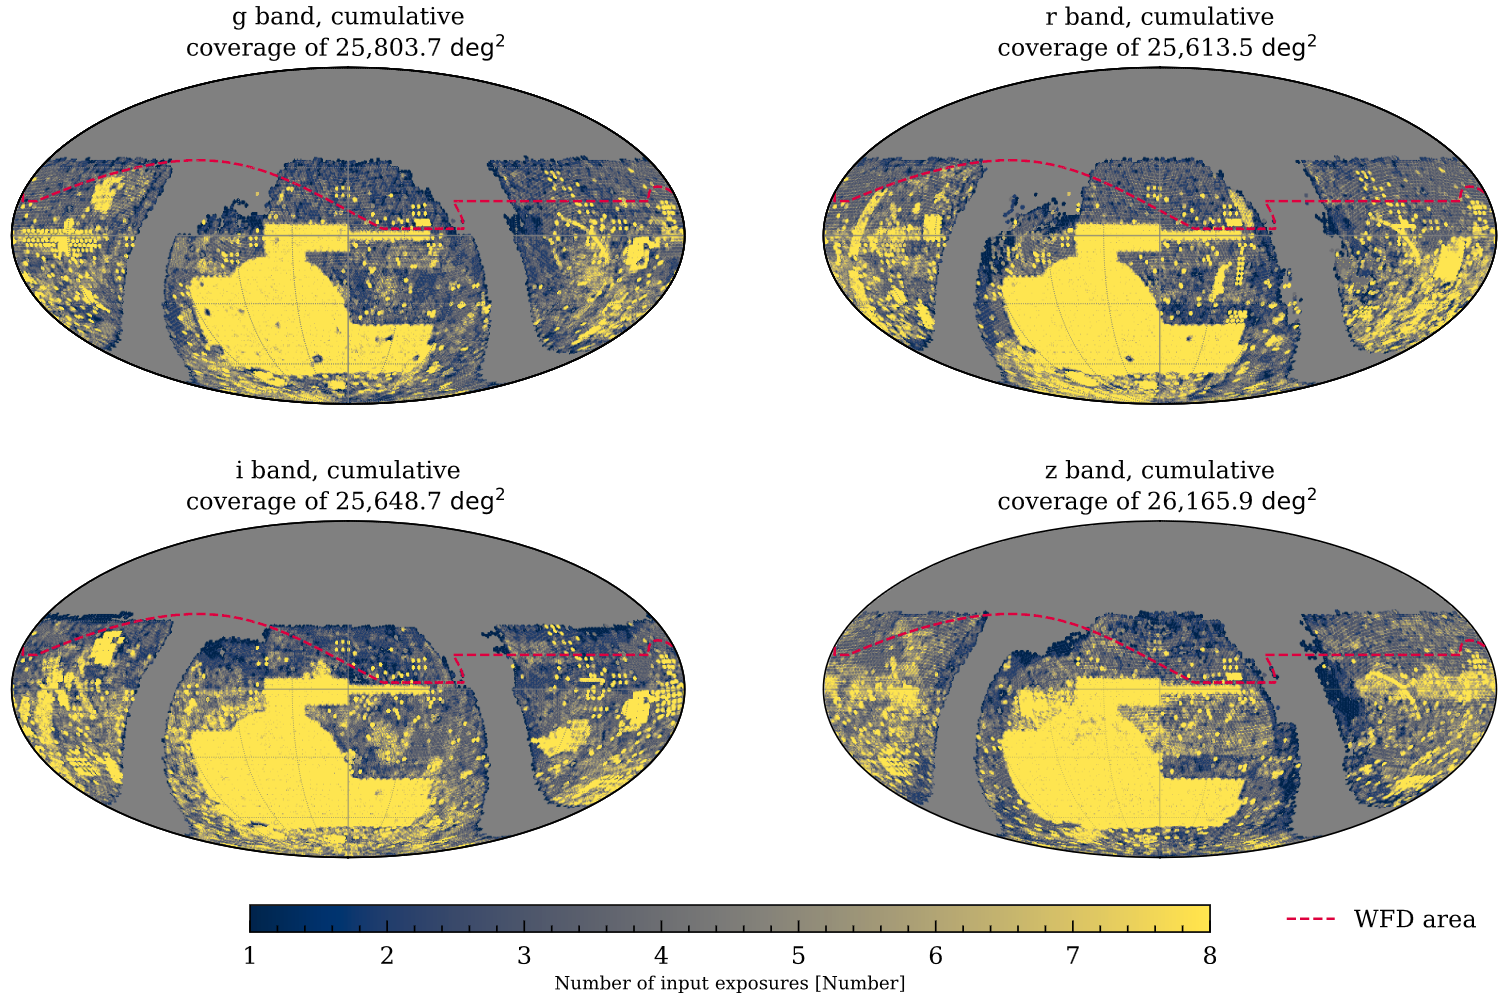
\includegraphics[width=0.99\linewidth]{figures/DELVE_vis_nomask.png}
    \caption{Input visits from DELVE DR3 shown per band, with the WFD northern declination limit shown in dashed red line.}
    \label{fig:delve_vis_nomask}
\end{figure}

\subsection{Band and footprint selection}

\textbf{Bands.} The campaign targets $griz$ only. The DELVE input lists are provided for these four bands. % DECam $u$-band data are sparse over most of the sky, and $Y$-band data exist almost exclusively in DES. Moreover, the DECam $u$-band system response differs appreciably from Rubin's, which would complicate its use even where data exist.

\textbf{Footprint.} Processing is limited to declinations south of approximately $+30^\circ$, which extends beyond the nominal Rubin wide-fast-deep and ecliptic regions so that templates would be available should LSST observations be taken outside the main footprint. A Galactic-latitude mask of $|b|>10^\circ$ is also applied to the DELVE inputs. Coverage was assessed against maps of where LSSTCam has accumulated enough images that templates could be built independent of this campaign already (\textit{incremental template maps}), so that DECam processing prioritizes regions in which LSSTCam templates are unlikely to be available. 

With these cuts, the potential template area is of order $6\times 10^4$\,deg$^2$ summed over $griz$, of which around $4\times 10^4$\,deg$^2$ is in seasonally prioritized regions, with a smaller requirement in $z$ band where Rubin already has substantial incremental template coverage. These estimates apply the general footprint cuts and do not yet fold in the true DELVE coverage, so the achievable area will be somewhat smaller.

% \sean{add a figure here showing the DECam coverage with the incremental mask applied}

Some regions are covered only partially or not at all by this input list. The Large and Small Magellanic Clouds are included in the input dataset. The part of the North Ecliptic Spur that passes through Orion and the Flame nebula is uncovered, but it suffers high extinction and has been de-prioritized by extragalactic surveys. Other DECam programs, such as DECaPS in the Galactic plane, provide additional images, but they would require different processing and are deferred until the present campaign is complete.

\subsection{Selection of exposures for each template}

Beyond the parent list, a visit-selection step in the template pipeline chooses the exposures that enter each template. The pipeline is derived from the base DECam \texttt{QuickTemplate} pipeline in \texttt{ap\_pipe}. Early tests used its default best-seeing selection. A quantile-based selector was initially adopted, with a maximum PSF FWHM of 1.8 arcsec, a minimum of eight visits, and a seeing quantile cut at 0.5. Experience showed that quantile-based selection has little effect until roughly ten or more images per band are available, and that DECam inputs per position are often too few for it to take effect, so the emphasis shifted from selecting the best fraction of inputs to simply rejecting poor ones.

The pilot compared three configurations: the earlier default selection, and a best-seeing selection of six exposures with a PSF cut at 1.8 arcsec and at 1.5 arcsec. Based on the PSF-variation metrics and difference-imaging tests, the campaign settled on the following rule: \textbf{each template is built from at most six DECam exposures, taken from the best-seeing exposures that satisfy a PSF cut of 1.5\,arcsec on the individual exposures}. A template is still built when fewer than six qualifying exposures exist, in which case all of them are used.

% \sean{Show plot comparing 1.8 and 1.5 arcsec template quality here}

These quality criteria are applied independently of those that will be used to select LSSTCam images for Rubin templates. The two sets of cuts are not coupled, and the DECam cuts should not be taken as a prediction of the LSSTCam template requirements.

\subsection{Calibration inputs for the selected exposures}

The selected exposures are reprocessed from raw images in the Rubin Science Pipelines. This replaces, rather than reuses, earlier DECam reductions such as the instrumental-signature-removed (instcal) images from the DECam Community Pipeline or the final-cut images from DES data management. Bad-pixel masks, the linearizer and other curated calibrations come from \texttt{obs\_decam}; the defects originate from DES.

Biases and flats were rebuilt from raw calibration exposures on a yearly epoch, and assembled with the pipeline's calibration-production tasks. Fringe frames are built after the $z$-band flats are validated. Because calibrations transferred between pipelines (or versions of the same pipeline) are unreliable, photometric zero points are not imported from DES or DELVE; instead, astrometry and photometry are calibrated against The Monster reference catalog within the Rubin pipeline \citep{DMTN-277}.

Calibration epochs were initially defined to follow a yearly cadence. However, work is ongoing to follow the DES and DECADE epochs, which are determined by instrumental features including power cycles and movements of the filters.

% Two known data issues are accommodated rather than corrected: the headers' read noise values were wrong by factors of roughly 1.5--2 on one backplane for an extended period (approximately 2014 to 2026), which has little effect on broad-band images of reasonable exposure time \todo{confirm the date range and which backplane}, and 
Edge bleeds were identified as a source of artifacts, for which a masking task was developed and validated against the DES edge-bleed mask, raising amplifier-level completeness from 63\% to 90\%. The brighter-fatter correction was judged unnecessary for template production, since the effect is small for this application.

\subsection{Curation and consistency with Rubin templates}

Each template is checked against PSF-variation metrics across tracts and bands before deployment, and the selection and vetting workflow is described in Section~\ref{sec:deployment}. Two curation rules are fixed in advance. First, within any tract and band, the official template collection used for real-time processing contains only one style of template, Rubin or DECam, never a mixture; this is enforced during curation using the expected Rubin coverage described above. Second, DECam templates are ingested under their own dataset type, \texttt{template\_coadd\_decam}, so that the provenance of every template is explicit. The instrument used in the coaddition is also recorded in the template metadata so that difference imaging and downstream products can identify which kind of template was used.


% ---------------------------------------------------------------------------
\begin{table}[t]
\centering
\small
\begin{tabular}{@{}p{0.15\textwidth}p{0.5\textwidth}p{0.25\textwidth}@{}}
\toprule
Stage & Criterion & Source \\  \hline  \hline
\midrule
Parent list & DELVE DR3 exposure list, $griz$ only & DELVE \\ \hline
% Homogenization & Low-quality exposures removed where exposures per band greatly exceed the typical depth (threshold of order 20) & DELVE \\
Exclusion & Known tracking, artifact and ghost-affected visits and CCDs & DELVE exclude list \\ \hline
Footprint & $\delta < +30^\circ$, Galactic-latitude mask, prioritized by expected LSSTCam template coverage & DELVE exposure list \\ \hline
Per-exposure quality & PSF cut of 1.5\,arcsec on individual exposures & Pilot comparison \\ \hline
Per-template selection & Up to six best-seeing exposures; fewer allowed & Pilot comparison \\ \hline
Calibration & Raw reprocessing, rebuilt calibrations by epoch, \textit{The Monster} for astrometry and photometry & Rubin Science Pipelines \\ \hline
Consistency & One template style per tract and band; \texttt{template\_coadd\_decam} dataset type & Deployment plan \\
\bottomrule
\end{tabular}
\caption{Summary of image selection and curation criteria.}
\label{tab:criteria}
\end{table}